%************AUSWERTUNG****************
\chapter{Results}
\section{Pentacenequinone}
In Figure \ref{fig:pentacenene} the STM Images of Pentacenequinone deposited on Ag(100) are shown.
It appears that PQ formes irregular shaped islands.
Also, the terasse edges appear  rough compared to Ag(100) terasse edges, indicating the presence of a PQ layer.
No smaller structures within the first layer or the island could be observed using STM, additionally LEED doesn't show any periodic structure.
It therefore can be concluded that PQ doesnt from any periodic structure on Ag(100), consequently the focus of this thesis lays on the study of 2HPc.
\duofigcom{C:\\Bac_Arbeit\\ratumi_bac\\bac_template\\graphics\\ready_images_pentacene\\41nm_pentacene_3dig.png}{fig:penta_3dig}{C:\\Bac_Arbeit\\ratumi_bac\\bac_template\\graphics\\ready_images_pentacene\\41nm_pentacene_1dig.png}{fig:penta_1dig}{1 Monolayer + 2nd layer islands of pentacenequinone on Ag(100) $U_{bias}$ = 2 mV , $I$ = 8 nA}{fig:pentacenene}

\newpage
\section{2-Hydrogen Phthalocyanin on Ag(100)}
\label{sec:results}The STM and LEED Images of 2-Hydrogen Phthalocyanin (2HPc) on Ag(100) show the Formation of an ordered and almost defect-free structure.
This indicates good mobility of the molecule during film growth.
As seen in the Image \ref{fig:2hpcphase} the 2HPc  arranges in $\sqrt{34} \times  \sqrt{34}\text{R}31$ phase with an relative rotation of the molecular axis (MA) in respect to the [010] direction of (11.6 $\pm$ 1.2)° (see figure \ref{fig:2hpcphase}). 
\monofig{width = 0.7\textwidth}{C:\\Bac_Arbeit\\ratumi_bac\\bac_template\\graphics\\ready_images_phthalo\\2Hpc_on_Ag100_3.PNG}{STM image of 2HPc/Ag(100) taken in constant-current mode (monolayer regime). Image of Ag(100) at the same scale as reference  . $U_{bias}$ = 480 mV , I = 0.05 nA. MA: Molecular axis. blue square: unit cell of $\sqrt{34} \times  \sqrt{34}\text{R}31$ phase}{fig:2hpcphase}  
\noindent %The Molecule itself appears as a 4-fold symmetric cross with a dark center in the middle or as 2-fold symmteric cross with two opposing isoindole units seeming brighter than the other two for negative polarity of the biasvoltage (filled-state imaging) . 
At positive biasvoltages close to the fermi edge 2HPc appears as a cross with two opposing isoindole unit seemingly brighter than the other two.
This is consistent with previous observation in literature for 2HPc on Ag(111), where the two bright isoindole units correspond to the two hydrogen atoms bound to the two pyrolic nitrogen atoms. \cite{sperl2011controlled}
At negative biasvoltages close to the fermi edge the 2HPc Molecules appear as crosses with two fold symmetry, where two opposing isoindole units exibit a different orbital structure than the other two. (see Figure \ref{fig:LUMO_1}).
This appearence is consistent with the 2HPc LUMO, calculated using DFT. \cite{database}
It is oriented in such a way that the benzene ring of one 2HPc molecule points towards the benzene ring of its nearest neighbor.
As seen in Fig. \ref{fig:LUMO_1} the LUMO can be observed near the Fermi Edge which suggests Fermi Level pinning.
\newpage
This is most likely due to fractional charge transfer from the metal substrate , leading to an partially occupied LUMO and thus a charged molecule.  
\duofigcom{C:\\Bac_Arbeit\\ratumi_bac\\bac_template\\graphics\\ready_images_phthalo\\2HPc_on_Ag100_LUMO_1.png}{fig:LUMO_1}{C:\\Bac_Arbeit\\ratumi_bac\\bac_template\\graphics\\ready_images_phthalo\\2Hpc_on_Ag100_LUMO_positive.PNG}{fig:HOMO_1}{(a) Constant-current image of 2Hpc/Ag(100). Two distinct LUMO orientations can be seen and their DFT-Simulation \cite{database} counterparts. U = -50.0 mV , I = 0.05 nA. (b) Same spot imaged in constant-current mode at positive Bias-Voltages. $U_{bias}$ = 750 mV , 0.02 nA.  }{}
\noindent In Figure \ref{fig:HOMO_1} the same area as in Figure \ref{fig:LUMO_1} is shown at large positive biasvoltage, revealing unoccupied states in form of a two fold symmetric orbital.
\begin{wrapfigure}{l}{0.6\textwidth}
    \centering
    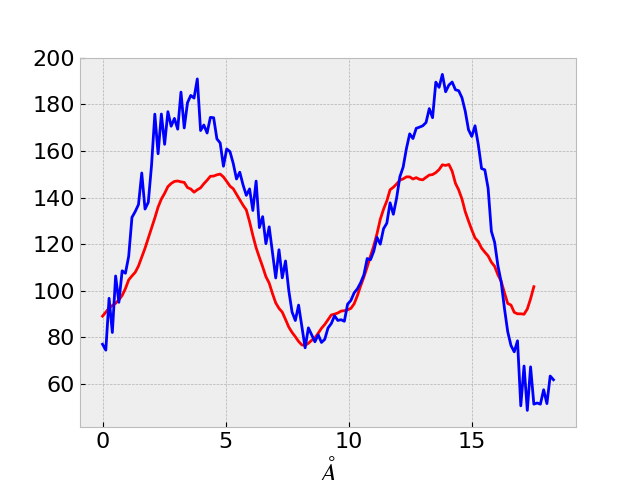
\includegraphics[width=0.6\textwidth]{graphics/ready_images_phthalo/profile_plot_2Hpc_on_Ag.png}
    \caption{
        Height profile plot,
        blue: vertical axis,
        red: horizontal axis}
    \label{fig:intensityAg}
\end{wrapfigure}
By looking at the pictures it is rather hard to see the brightness difference between the two pairs of isoindole units. 
In Fig \ref{fig:intensityAg} the intensity profile of the two perpendicular axis of the molecule shown in Fig \ref{fig:HOMO_1} were investigated, which show significant brightness difference in the benzene ring locations.
It is notable that the LUMOs axis is flipped 90° for some molecules when switching the polarity of the biasvoltage.
There are two degenerated LUMOs, with the electron density concentrated around two opposing isoindole units. 
This makes the Molecule reduce its symmetry from 4-fold to 2-fold.
There is no favored orientation seen in the STM images, which suggest that the occupation probability of the two LUMOs is the same. 



\section{Magnesium-Oxide (MgO)}
Before depositing 2HPc (2H-phthalocyanine) on a MgO thin film, the quality of the surface was assessed using scanning tunneling microscopy (STM), followed by capturing a low-energy electron diffraction (LEED) image.
The MgO forms sharp rectangular Islands with the edges along the [011] and [01$\bar{1}$] directions as expected.
In Figure \ref{fig:21nm_mgo} it can be seen that most of the islands are 15 - 20 nm wide.
The Images show a MgO film consistent with literature.\cite{articlemgo}
%\duofigcom{C:\\Bac_Arbeit\\ratumi_bac\\bac_template\\graphics\\ready_images_MgO\\21nm_MgO.png}{fig:21nm_mgo}{C:\\Bac_Arbeit\\ratumi_bac\\bac_template\\graphics\\ready_images_MgO\\10nm_MgO.png}{fig:10nm_mgo}{Both (a) and (b) taken at 3.5 V Biasvoltage, most likely sub-monolayer to monolayer regime}{}
\monofig{width = 0.7\textwidth}{C:\\Bac_Arbeit\\ratumi_bac\\bac_template\\graphics\\ready_images_MgO\\21nm_MgO.png}{Image taken at $U_{bias}$ 3.5 V, most likely sub-monolayer to monolayer regime}{fig:21nm_mgo}
\newpage
\section{2-Hydrogen Phthalocyanine on MgO}
The STM images of 2HPc on MgO(100)/Ag(100) show again the formation of an ordered structure that persists across the the whole crystal lattice.
Evident is the presence of linear defects, on which sites the 2HPc phase is shifted or even disconnected. 
This is most likely due to the fact that the underlying MgO long-range order is disturbed by the 3.2 \% mismatch of the Ag an MgO lattice.
Therefore resulting in incoherent sites, which give rise to intermediate phases with different orientation.
In figure \ref{fig:2hpcMgO} the phase of the molecular adsorbate was determined.
This was done using the Ag(100) lattice vectors, as they are almost identical to the MgO lattice.
The superstructure of 2HPc on MgO(100)/Ag(100) was determined using a combination of STM and LEED measurements.
The unit cell of 2HPc on MgO is rotated in direction of the [01$\bar{1}$] plane and is also larger than on Ag which can be attributed to the larger lattice constant.
The phase was estimated to $\sqrt{40} \times  \sqrt{40}\text{R}18.4$ .
In contrast to 2HPc on Ag(100) the molecule is mirrored in respect to the [001] plane with an molecular axis angle of (1.9 $\pm$ 1.4)°.
\monofig{width = 0.7\textwidth}{C:\\Bac_Arbeit\\ratumi_bac\\bac_template\\graphics\\ready_images_phthalo\\2Hpc_on_MgO_2.PNG}{STM image of 2HPc on Mg0(100)/Ag(100) taken in constant-current mode (monolayer regime). Image of Ag(100) at the same scale as reference . U = 200 mV , I = 1 nA. MA: Molecular axis. blue square: unit cell of $\sqrt{40} \times  \sqrt{40}\text{R}18.4$ phase}{fig:2hpcMgO}  
\noindent
For further verification of the observed structure a LEED picture at 15 eV was taken after analysis with the STM.
The LEED clearly supports the mainly observed phase, but appeared diffuse which can come from additional phases or additional diffraction caused by the molecular structure.
Additionally a 2D-FFT was performed on the STM image in figure \ref{fig:2hpcMgO} ,which aligns nicely with the observed LEED image.
\duofigcom{C:\\Bac_Arbeit\\ratumi_bac\\bac_template\\graphics\\ready_images_phthalo\\2HPc_on_MgO_FFT.JPG}{fig:2hpcMgoFFT}{C:\\Bac_Arbeit\\ratumi_bac\\bac_template\\graphics\\ready_images_phthalo\\2HPc_on_MgO_LEED.PNG}{fig:2hpcMgoLEED}{(a) 2D-FFT of image in \ref{fig:2hpcMgO}, (b) LEED picture taken at $E_{kin}$ = 15 eV}{fig:fftnLEED}
\monofig{width=0.7\textwidth}{ready_images_phthalo\\multiple.png}{Additional phases observed for 2HPc on MgO(100)/Ag(100). }{fig:multiple}
\noindent As seen in Fig. \ref{fig:multiple} there are three additional phases with two of them (red and green) aligned at the high symmetry direction [110], but different molecular orientation.
The unit cells all have the same size. 
\duofigcom{C:\\Bac_Arbeit\\ratumi_bac\\bac_template\\graphics\\ready_images_phthalo\\2HPc_on_MgO_neg_250mV_rings_axis.PNG}{fig:onMgo400mV}{C:\\Bac_Arbeit\\ratumi_bac\\bac_template\\graphics\\ready_images_phthalo\\2HPc_on_MgO_700mV_rings.PNG}{fig:onMgO700mV}{(a) Image taken of a charged molecule at $U_{bias}$ = -250 mV $I$ = 0.06 nA , (b) charged molecule clusters at $U_{bias}$ = 700 mV , $I$ = 0.07 nA }{fig:onMgO}
\begin{wrapfigure}{l}{0.6\textwidth}
    \centering
    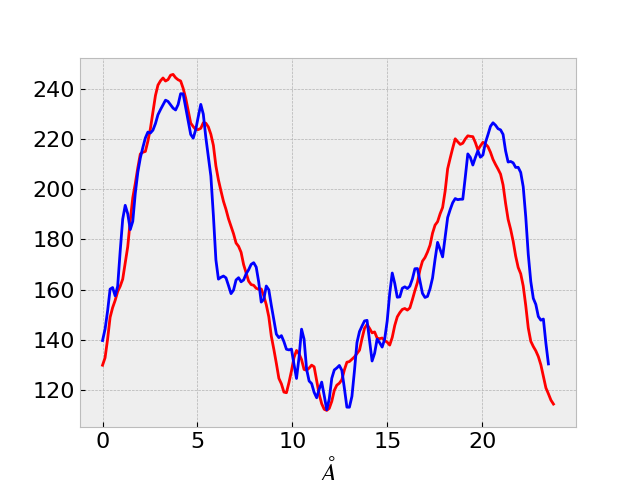
\includegraphics[width=0.6\textwidth]{graphics/ready_images_phthalo/profile_plot_2Hpc_on_mgo.png}
    \caption{
        Intesity profile plot,
        blue: vertical axis,
        red: horizontal axis}
    \label{fig:intensitymgo}
\end{wrapfigure}
\noindent The image depicted in Figure \ref{fig:onMgo400mV} was captured below the Fermi Energy level. 
It appears to feature a singly charged molecule, despite lacking the anticipated 2-fold symmetry observed in the calculated LUMO.
This cannot be easily explained with the available data.
These "rings" are also seen for distinct positive bias voltages, which indicates SOMO/SUMO splitting of the molecules LUMO.
%This is also supported by Scanning Tunneling Spectroscopy performed on the "ring" parts of the electronic structure ,which shows two distinct peaks asymmetricly around the the Fermi Edge.  
These two secluded states are seen for biasvoltages greater than 430 mV and less than -250 mV. 
Further investigation is needed to fully understand these complex electronic structures.
